\chapter{Portraits de phases de systèmes linéaires}\label{chap:portrait_phases}
    \section{Introduction}
        \begin{definition}{Portrait de phases}
            Le portrait de phases est une représentation graphique qui fournit une vue d'ensemble du comportement qualitatif d'un système dynamique en visualisant l'évolution de ses trajectoires dans l'espace des phases.
        \end{definition}
        Il permet d'observer les attracteurs, les cycles limites, les points d'équilibre, ainsi que les directions et les tendances globales du système, offrant ainsi un aperçu des propriétés structurelles et de la stabilité des solutions sans nécessiter la résolution explicite des équations différentielles. Un exemple est donné en figure \ref{fig:exemple_portrait_de_phases}, pour un système décrit par la matrice
        \begin{equation}
            A = \begin{bmatrix}1 & -2\\-3 & 1\end{bmatrix}
        \end{equation}
        où l'on voit clairement que le système à un comportement de \textit{selle} autour du point d'équilibre.

        \begin{figure}[ht!]
            \centering
            \includegraphics[width=\textwidth]{images/exemple_portrait_de_phases.jpg}
            \caption{Exemple de portrait de phases}
            \label{fig:exemple_portrait_de_phases}
        \end{figure}

        L'étude et le dessin des portraits de phases est un sujet autant complexe qu'il existe une infinité de systèmes possibles. Dans ce chapitre, nous nous concentrerons sur les systèmes d'équations différentielles d'ordre 2. Nous commençons par présenter de manière extensive les cas envisageables, en montrant les méthodes de résolutions et en amenant des cas par des exercices à réaliser sur papier. Dans la suite du chapitre, à la section \ref{sec:poincare}, nous présenterons la relation entre tous les comportements du système et la localisation de ce système dans le \textit{diagramme de Poincaré}, ce qui permettra d'accélérer nettement l'évaluation du comportement du système. 

        Nous pensons qu'il est indispensable de construire une intuition du comportement des systèmes autour des points d'équilibre pour bien comprendre, et non pas retenir, la construction de ce diagramme de Poincaré. La confrontation aux exemples avant la présentation d'une méthode plus générale conviendra aux étudiant·e·s qui préfèrent généraliser par l'exemple. Sinon, la section \ref{sec:poincare} présente ce diagramme, et peut être abordé avant d'étudier chaque cas individuellement. Nous insistons néanmoins sur la nécessité d'étudier chaque type de comportement individuellement, car chacun a ses subtilités de calcul qui doivent être explorées.
    
    \section{Points d'équilibre et stabilité}
        \begin{definition}{Point d'équilibre}
            Un point d'équilibre (ou \textit{point fixe}) est un point à partir duquel la trajectoire coïncide avec la condition initiale.
        \end{definition}
         Il répond à la condition $\dot{x} = 0$, étant donné que sa variation doit être nulle. Si $A$ est la matrice des coefficients du système étudié, et que $\det(A) \neq 0$, alors le seul état d'équilibre est $(0, 0)$. \robin{La caractérisation des solutions aux systèmes linéaires a été vue en F205, ça doit donc être connu ici} Sinon, il en existe d'autres.
         Une fois le(s) point(s) d'équilibre déterminés, on peut étudier la notion de stabilité. Comme vu au cours théorique, on dit qu'une trajectoire est \textit{stable} selon le critère de Liapounov si, pour tout point initial proche de cette trajectoire, les trajectoires qui en résultent restent dans un voisinage suffisamment petit autour de l'orbite au fil du temps. Autrement dit, si l'on perturbe légèrement un point sur cette orbite, la trajectoire de ce point perturbé restera à proximité de l'orbite initiale au lieu de s'en écarter indéfiniment. 

        \begin{definition}{Système stable}
            Un système dynamique linéaire est dit \textbf{stable} si son mouvement libre est limité pour chaque valeur de la condition initiale.
        \end{definition}

        \begin{definition}{Système asymptotiquement stable}
            Un système dynamique linéaire est dit \textbf{asymptotiquement stable} si son mouvement libre tend vers le point d'équilibre pour $t \to \infty$ pour chaque valeur de la condition initiale.
        \end{definition}

        \begin{definition}{Système instable}
            Un système dynamique linéaire est dit \textbf{instable} s'il existe au moins une condition initiale telle que le mouvement libre qui en suit est non limité.
        \end{definition}

        On peut distinguer des cas plus précis, qui dépendent du type et du signe des valeurs propres du système que l'on regarde. 
        Si les deux valeurs propres sont réelles et négatives, l'état d'équilibre est stable et est appelé un \textit{nœud stable}. Si les deux valeurs propres sont réelles et positives, l'état d'équilibre est instable et est appelé un \textit{nœud instable}. Si l'une est positive et l'autre négative, l'état d'équilibre est instable et est appelé une \textit{selle}. Ces différents cas seront présentés plus en détail.

    
    \section{Les vecteurs vitesse}
        Soit le système
        \begin{equation}
            \dot{x} = A x
        \end{equation}
        avec 
        \begin{equation}
            A = \begin{bmatrix} -2 & 1 \\ 1 & -2 \end{bmatrix}
        \end{equation}
        Soit un instant $t$ tel que l'état $x = \begin{bmatrix} 0.5 \\ 0 \end{bmatrix}$. Le vecteur vitesse à cet état est défini en résolvant le système d'équations différentielles \robin{Ce n'est pas un système d'équations différentielles~: $t$ est fixé, on cherche juste à résoudre un système linéaire dans $\mathbb R$}, par
        \begin{equation}
            \begin{bmatrix} \dot{x}_1 \\ \dot{x}_2 \end{bmatrix} = A \begin{bmatrix} 0.5 \\ 0 \end{bmatrix}
        \end{equation}
        Ce vecteur donne le sens, la direction et la vitesse de la trajectoire à notre état $\begin{bmatrix}x_1\\ x_2\end{bmatrix}$. Calculons le vecteur vitesse :
        \begin{equation}
            \begin{cases}
                \dot{x}_1 = -2x_1 + x_2 = -1\\
                \dot{x}_2 = x_1 - 2x_2 = 0.5
            \end{cases}
        \end{equation}
        Le vecteur vitesse est donc $\dot{x} = \begin{bmatrix} -1\\ 0.5\end{bmatrix} $.
        Calculons le vecteur vitesse au point $x = \begin{bmatrix} -0.5 \\ -1 \end{bmatrix}$ :
        \begin{equation}
            \begin{cases}
                \dot{x}_1 = -2x_1 + x_2 = 0 \\
                \dot{x}_2 = x_1 - 2x_2 = 1.5
            \end{cases}
        \end{equation}
        Le vecteur vitesse est donc $\dot{x} = \begin{bmatrix} 0\\ 1.5\end{bmatrix} $. 
        Avec cette méthode, on peut déterminer le vecteur vitesse en tout point du plan \robin{de l'espace des phases. Ici c'est un plan, mais ça fonctionne conceptuellement en dimension arbitraire}. 
        
        Si l'on trace les vecteurs vitesse pour un ensemble suffisamment grand de points, on obtient une première estimation du comportement du système, comme montré dans la figure \ref{fig:vecteurs_vitesse} pour le système décrit par la matrice 
        \begin{equation}
            A = \begin{bmatrix}1 & -2\\-2 & 1\end{bmatrix}
        \end{equation}
        Cette visualisation peut être obtenue grâce au code python suivant :
        \inputminted{python}{codes/vecteurs_vitesse.py}
        
        \begin{figure}[ht!]
            \centering
            \includegraphics[width=\textwidth]{images/vecteurs_vitesse.jpg}
            \caption{Exemple de vecteurs vitesse}
            \label{fig:vecteurs_vitesse}
        \end{figure}

    
    \section{Valeurs propres et vecteurs propres}
        Calculons les valeurs propres du système décrit par $A$:
        \begin{equation}
            \begin{split}
            \det(A - \lambda I) &= 0 \\
            \Rightarrow \lambda^2 + 4\lambda + 3 &= 0\\
            \lambda_{1,2} = -4 \pm \sqrt{4} &= \{-1, -3\}
            \end{split}
        \end{equation}
        Calculons ses vecteurs propres :
        \begin{equation}
            \begin{split}
                &(A - \lambda_1 I)\overrightarrow{v_1} = 0 \\
                \Rightarrow& \begin{bmatrix} -1 & 1 \\ 1 & -1 \end{bmatrix} \begin{bmatrix} x \\ y \end{bmatrix} = \begin{bmatrix} 0 \\ 0 \end{bmatrix}\\
                \Rightarrow& \begin{bmatrix} x \\ y \end{bmatrix} = k \cdot \begin{bmatrix} 1 \\ 1 \end{bmatrix} \quad \forall k \\
                \Rightarrow& \overrightarrow{v_1} = \begin{bmatrix} 1 \\ 1 \end{bmatrix}
            \end{split}
        \end{equation}
        et pour $\lambda_2$,
        \begin{equation}
            \begin{split}
                &(A - \lambda_2 I)\overrightarrow{v_2} = 0 \Rightarrow \begin{bmatrix} 1 & 1 \\ 1 & 1 \end{bmatrix} \begin{bmatrix} x \\ y \end{bmatrix} = \begin{bmatrix} 0 \\ 0 \end{bmatrix}\\
                \Rightarrow& \begin{bmatrix} x \\ y \end{bmatrix} = k \cdot \begin{bmatrix} 1 \\ -1 \end{bmatrix} \quad \forall k \\
                \Rightarrow& \overrightarrow{v_2} = \begin{bmatrix} 1 \\ -1 \end{bmatrix}
            \end{split}
        \end{equation}

        De nouveau, il est possible de calculer ces vecteurs propres numériquement en python, grâce au code suivant:
        \inputminted{python}{codes/vecteurs_propres.py}
        Et le résultat peut être affiché comme montré dans la figure \ref{fig:vecteurs_propres}.
        \begin{figure}[ht!]
            \centering
            \includegraphics[width=\textwidth]{images/vecteurs_propres.jpg}
            \caption{Exemple de vecteurs vitesse \robin{Ce sont les vecteurs propres ici, pas les vecteurs vitesse}}
            \label{fig:vecteurs_propres}
        \end{figure}
        
        Notez bien que tout vecteur qui est un multiple de l'un des vecteurs propres que nous avons calculés est encore un vecteur propre.
        Prenons un état correspondant à un multiple du vecteur propre $\overrightarrow{v_1} = \begin{bmatrix} 1 \\ 1 \end{bmatrix}$, par exemple $\begin{bmatrix}2\\ 2\end{bmatrix}$, et calculons son vecteur vitesse :
        \begin{equation}
            \begin{cases}
                \dot{x}_1 = -2x_1 + x_2 = -2 \\
                \dot{x}_2 = x_1 - 2x_2 = -2
            \end{cases}
        \end{equation}
        Le vecteur vitesse est donc $\begin{bmatrix}-2\\ -2\end{bmatrix}$. Notez que le déplacement reste dans la même direction que notre vecteur vitesse initial.

        En règle générale : si on part d'un état $v$ qui est un multiple d'un vecteur propre, le vecteur vitesse a la même direction que ce vecteur propre.
        
        Cette règle est vérifiable formellement. Soit une paire de vecteur et valeur propre $(v, \lambda)$. Nous avons par définition
        \begin{equation}
            A v = \lambda v
        \end{equation}
        et donc, en revenant au système, si on part d'un état $x = k \cdot v$, nous avons
        \begin{equation}
            \begin{split}
                &\dot{x} = A x \\
                \Rightarrow& \dot{x} = k A v = k \lambda v
            \end{split}
        \end{equation}
        Nous voyons donc que le vecteur vitesse $\dot{x}$ est bien un multiple du vecteur propre $v$.
    \section{Exercices}
        Comme dans le chapitre sur la résolution d'équations différentielles, on vous donne un système d'équations différentielles d'ordre 2, de la forme \robin{Tu utilises $A_{ij}$ (en majuscule) alors que tu utilisais $a_{ij}$ dans le chapitre précédent}
        \begin{equation}
            \begin{cases}
                \dot{x}_1(t) = A_{00} x_1(t) + A_{01} x_2(t)\\
                \dot{x}_2(t) = A_{10} x_1(t) + A_{11} x_2(t)
            \end{cases}
        \end{equation}
        Vous devez:
        \begin{enumerate}
            \item définir la matrice des coefficients~;
            \item définir l'équation caractéristique~;
            \item calculer les valeurs propres~;
            \item déterminer les vecteurs propres, et les trajectoires associées~;
            \item dessiner les vecteurs vitesses pour des points bien choisis~;
            \item dessiner la trajectoire du système pour ces conditions initiales pour un intervalle de temps donné.
        \end{enumerate}
        Ces exercices sont à réaliser à la main, sur papier millimétré. Afin d'offrir une auto-vérification, nous proposons les solutions générées par le code suivant:
        \inputminted{python}{codes/correction_pdp_1.py}
        
        \subsection{Exercice 1: nœud stable}
            \begin{exercise}{Nœud stable}
                Effectuez les étapes présentées à la section précédente pour le système
                \begin{equation}
                    \begin{cases}
                        \dot{x}_1(t) = x_1(t) - 2 x_2(t)\\
                        \dot{x}_2(t) = - 2 x_1(t) + x_2(t)
                    \end{cases}
                \end{equation}
            \end{exercise}
            Tracez les vecteurs vitesses en $x = \begin{bmatrix}1 \\ 1\end{bmatrix}$, $\begin{bmatrix}-1 \\ 1\end{bmatrix}$, $\begin{bmatrix}1 \\ -1\end{bmatrix}$ et $\begin{bmatrix}-1 \\ -1\end{bmatrix}$, et en $x = \begin{bmatrix}0 \\ 1\end{bmatrix}$, $\begin{bmatrix}1 \\ 0\end{bmatrix}$, $\begin{bmatrix}0 \\ -1\end{bmatrix}$ et $\begin{bmatrix}-0.5 \\ -1\end{bmatrix}$. Tracez les trajectoires démarrant en $x = \begin{bmatrix}0 \\ 1\end{bmatrix}$ et en $x = \begin{bmatrix}-0.5 \\ -1\end{bmatrix}$.
            La solution numérique est donnée en figure \ref{fig:pdp_exercice_1}.
            \begin{figure}[ht!]
                \centering
                \includegraphics[width=\textwidth]{images/pdp_exercice_1.jpg}
                \caption{Solution numérique de l'exercice 1}
                \label{fig:pdp_exercice_1}
            \end{figure}
                
        \subsection{Exercice 2: nœud instable}
            \begin{exercise}{Nœud instable}
                Effectuez les étapes présentées à la section précédente pour le système
                \begin{equation}
                    \begin{cases}
                        \dot{x}_1(t) = 2 x_1(t) + x_2(t)\\
                        \dot{x}_2(t) = 2 x_1(t) + 3 x_2(t)
                    \end{cases}
                \end{equation}
            \end{exercise}
            Tracez les vecteurs vitesses en $x = \begin{bmatrix}0.5 \\ 1\end{bmatrix}$, $\begin{bmatrix}-0.5 \\ -1\end{bmatrix}$, $\begin{bmatrix}-1 \\ 1\end{bmatrix}$ et $\begin{bmatrix}1 \\ -1\end{bmatrix}$, et en $x = \begin{bmatrix}0 \\ 1\end{bmatrix}$, $\begin{bmatrix}1 \\ 0\end{bmatrix}$, $\begin{bmatrix}0 \\ -1\end{bmatrix}$ et $\begin{bmatrix}-0.5 \\ -1\end{bmatrix}$. Tracez les trajectoires démarrant en $x = \begin{bmatrix}0 \\ 1\end{bmatrix}$ et en $x = \begin{bmatrix}-0.5 \\ -1\end{bmatrix}$.
            La solution numérique est donnée en figure \ref{fig:pdp_exercice_2}.
            \begin{figure}[ht!]
                \centering
                \includegraphics[width=\textwidth]{images/pdp_exercice_2.jpg}
                \caption{Solution numérique de l'exercice 2}
                \label{fig:pdp_exercice_2}
            \end{figure}
        
        \subsection{Exercice 3: selle}
            \begin{exercise}{Selle}
                Effectuez les étapes présentées à la section précédente pour le système
                \begin{equation}
                    \begin{cases}
                        \dot{x}_1(t) = 5 x_1(t) + 9 x_2(t)\\
                        \dot{x}_2(t) = 6 x_1(t) + 2 x_2(t)
                    \end{cases}
                \end{equation}
            \end{exercise}
            Tracez les vecteurs vitesses en $x = \begin{bmatrix}1 \\ \frac23\end{bmatrix}$, $\begin{bmatrix}-1 \\ -\frac23\end{bmatrix}$, $\begin{bmatrix}-1 \\ 1\end{bmatrix}$ et $\begin{bmatrix}1 \\ -1\end{bmatrix}$, et en $x = \begin{bmatrix}0 \\ 1\end{bmatrix}$, $\begin{bmatrix}1 \\ 0\end{bmatrix}$, $\begin{bmatrix}0 \\ -1\end{bmatrix}$ et $\begin{bmatrix}-0.5 \\ -1\end{bmatrix}$. Tracez les trajectoires démarrant en $x = \begin{bmatrix}0 \\ 1\end{bmatrix}$ et en $x = \begin{bmatrix}-0.5 \\ -1\end{bmatrix}$.
            La solution numérique est donnée en figure \ref{fig:pdp_exercice_3}.
            \begin{figure}[ht!]
                \centering
                \includegraphics[width=\textwidth]{images/pdp_exercice_3.jpg}
                \caption{Solution numérique de l'exercice 3}
                \label{fig:pdp_exercice_3}
            \end{figure}
   \section{Systèmes non-simples}
        Dans cette section, nous étudions les portraits de phases des systèmes non-simples en analysant les différents types de valeurs propres et leurs implications sur la stabilité et les trajectoires dans le plan de phase. Nous considérons le système décrit par la matrice
        \begin{equation}
            A = \begin{bmatrix}
                a & b\\
                c & d
            \end{bmatrix}
        \end{equation}

        \subsection{Valeur propre nulle}
            Dans ce cas, où $\det A = 0$ avec $\lambda_1 = 0$, les états d'équilibre se trouvent sur la droite définie par :
            \begin{equation}
            ax_1 + bx_2 = 0,
            \end{equation}
            et les trajectoires suivent des droites parallèles dans la direction du vecteur propre associé $\mathbf{v}_2$. \robin{Notation de vecteur en gras alors que notation $\overrightarrow \cdot$ dans le chapitre précédent.} On distingue deux cas selon le signe de $\lambda_2$ :
            
            \begin{itemize}
                \item \textbf{Si $\lambda_2 < 0$ :} Les états d'équilibre sont stables, car toutes les trajectoires convergent vers la droite d'équilibre. \\
                \textit{Exemple :} $\lambda_1 = 0$, $\lambda_2 = -1$.
                
                \item \textbf{Si $\lambda_2 > 0$ :} Les états d'équilibre sont instables, car les trajectoires s'éloignent de la droite d'équilibre. \\
                \textit{Exemple :} $\lambda_1 = 0$, $\lambda_2 = 1$.
            \end{itemize}

        \subsection{Valeurs propres réelles et non-distinctes}
            Nous examinons ici le cas où $\lambda_1 = \lambda_2 = \lambda$, qui conduit à deux configurations selon la diagonalisabilité de $A$ :

            \begin{itemize}
                \item \textbf{Matrice $A$ diagonalisable :} Lorsque $A$ admet une infinité de vecteurs propres, chaque droite passant par l'origine est une trajectoire, et l'origine devient un \textit{nœud singulier}. Par exemple, le système décrit par la matrice
                \begin{equation}
                    A = \begin{bmatrix} -1 & 0 \\ 0 & -1 \end{bmatrix}
                \end{equation}
                décrit effectivement un nœud singulier, comme montré dans la figure \ref{fig:noeud_singulier}.
                \begin{figure}[ht!]
                    \centering
                    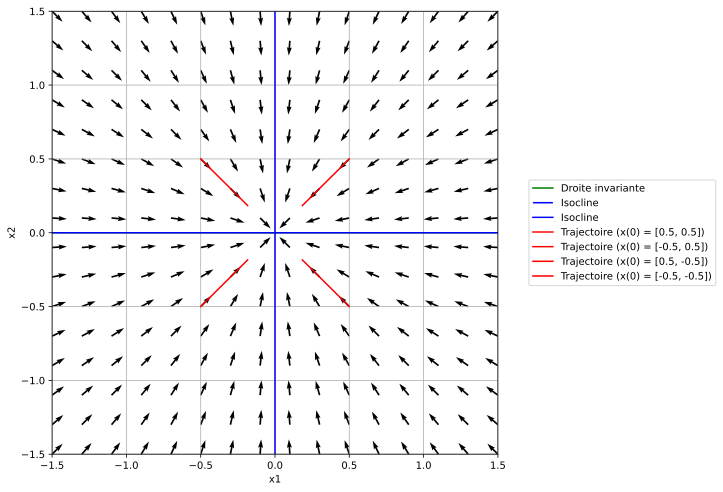
\includegraphics[width=\textwidth]{images/noeud_singulier.jpg}
                    \caption{Exemple de nœud singulier}
                    \label{fig:noeud_singulier}
                \end{figure}
                \begin{itemize}
                    \item Si $\lambda < 0$, le système est asymptotiquement stable.
                    \item Si $\lambda > 0$, le système est instable.
                    \item Si $\lambda = 0$, le système est simplement stable.
                \end{itemize}
            
                \item \textbf{Matrice $A$ non-diagonalisable :} Dans ce cas, $A$ n'a qu'un seul vecteur propre, et donc une seule direction possède une trajectoire rectiligne, tandis que les autres trajectoires prennent une forme parabolique. L'origine est alors un \textit{nœud dégénéré}. Par exemple, le système décrit par la matrice
                \begin{equation}
                    A = \begin{bmatrix} 3 & -4 \\ 1 & -1 \end{bmatrix}
                \end{equation}
                décrit effectivement un nœud dégénéré, comme montré dans la figure \ref{fig:noeud_degenere}.
                \begin{figure}[ht!]
                    \centering
                    \includegraphics[width=\textwidth]{images/noeud_degenere.jpg}
                    \caption{Exemple de nœud dégénéré}
                    \label{fig:noeud_degenere}
                \end{figure}
                Si $\lambda = 0$, toutes les trajectoires se trouvent sur des droites parallèles, comme montré dans la figure \ref{fig:mouvement_uniforme} pour le système décrit par la matrice
                \begin{equation}
                    A = \begin{bmatrix} 1 & 0 \\ 1 & 0 \end{bmatrix}
                \end{equation}
                \begin{figure}[ht!]
                    \centering
                    \includegraphics[width=\textwidth]{images/mouvement_uniforme.jpg}
                    \caption{Exemple de mouvement uniforme}
                    \label{fig:mouvement_uniforme}
                \end{figure}
            \end{itemize}

        \subsection{Valeurs propres complexes}
            Enfin, nous examinons le cas où les valeurs propres sont complexes : $\lambda_1 = a + ib$ et $\lambda_2 = a - ib$. Ici, la nature des trajectoires dépend du signe de la partie réelle $a$ :
            
            \begin{itemize}
                \item \textbf{Si $a = 0$ :} Les trajectoires forment des ellipses fermées avec une période de rotation $T = \frac{2 \pi}{|b|}$. L'origine est un \textit{centre}. Un exemple est montré en figure \ref{fig:centre}, avec la matrice
                \begin{equation}
                    A = \begin{bmatrix} 0 & 1 \\ -1 & 0 \end{bmatrix}
                \end{equation}
                \begin{figure}[ht!]
                    \centering
                    \includegraphics[width=\textwidth]{images/centre.jpg}
                    \caption{Exemple de centre}
                    \label{fig:centre}
                \end{figure}
                
                \item \textbf{Si $a < 0$ :} Le système est asymptotiquement stable, et les trajectoires convergent vers l'origine en spirale. L'origine est un \textit{foyer stable}. Un exemple est donné en figure \ref{fig:foyer_stable}, avec la matrice
                \begin{equation}
                    A = \begin{bmatrix} 0 & 1 \\ -1 & 1 \end{bmatrix}
                \end{equation}
                \begin{figure}[ht!]
                    \centering
                    \includegraphics[width=\textwidth]{images/foyer_stable.jpg}
                    \caption{Exemple de foyer stable}
                    \label{fig:foyer_stable}
                \end{figure}
                
                \item \textbf{Si $a > 0$ :} Le système est instable, et les trajectoires divergent de l'origine en spirale. L'origine est un \textit{foyer instable}. Un exemple est donné en figure \ref{fig:foyer_instable}, avec la matrice
                \begin{equation}
                    A = \begin{bmatrix} 0 & 1 \\ -1 & -1 \end{bmatrix}
                \end{equation}
                \begin{figure}[ht!]
                    \centering
                    \includegraphics[width=\textwidth]{images/foyer_instable.jpg}
                    \caption{Exemple de foyer instable}
                    \label{fig:foyer_instable}
                \end{figure}
            \end{itemize}
            
            La direction de rotation (horaire ou anti-horaire) des trajectoires autour de l'origine dépend du signe de la partie imaginaire $b$ des valeurs propres.
            
    \section{Diagramme de Poincaré}\label{sec:poincare}
        L'étude de la stabilité des systèmes dynamiques linéaires a bénéficié des contributions pionnières de Henri Poincaré, mathématicien du XIX\textsuperscript{e} siècle, dont les travaux ont permis d'approfondir la compréhension des systèmes dynamiques et du comportement de leurs points d'équilibre. Le diagramme de Poincaré, qui relie la trace et le déterminant d'une matrice à la nature des points d'équilibre, est aujourd'hui un outil fondamental pour la classification de la stabilité des systèmes dynamiques linéaires. Cette approche permet de prédire rapidement la stabilité d'un système, en offrant une visualisation claire des régions de stabilité et d'instabilité sur le plan des valeurs propres.
        
        \subsection{Trace et déterminant de la matrice $A$}
            La classification des points d'équilibre d'un système linéaire peut ainsi être résumée de manière compacte en utilisant la trace et le déterminant de la matrice $A$. En effet, les valeurs propres de $A$, notées $\lambda_1$ et $\lambda_2$, sont notamment calculables par l'expression
            \begin{equation}
                \lambda_{1,2} = \frac{\Tr(A) \pm \sqrt{\Tr(A)^2 - 4 \det(A)}}{2}
            \end{equation}
            obtenue en développant l'équation caractéristique (voir équation \ref{eq:equation_caracteristique}).
            
            Cette formule utilise deux éléments que nous savons calculer facilement depuis l'équation \ref{eq:valeurs_propres}: la trace $\Tr(A)$ et le déterminant $\det(A)$ de la matrice $A$. Ceux-ci permettent de déterminer la nature des valeurs propres, qu'elles soient réelles ou complexes, positives ou négatives, montrant ainsi la stabilité des points d'équilibre associés. En particulier, le discriminant 
            \begin{equation}
                \Tr(A)^2 - 4 \det(A) = 0
            \end{equation}
            définit une parabole sur le plan $(\Tr(A), \det(A))$ qui sépare différentes régions de stabilité dans le système dynamique. Cette parabole représente la transition entre les valeurs propres réelles et complexes, et sa position est cruciale pour interpréter les comportements qualitatifs des trajectoires. 

            Le diagramme de Poincaré, montré dans la figure \ref{fig:poincare}, présente cette classification en fonction de la trace et du déterminant de $A$, indiquant les différentes régions de stabilité et le type de points d'équilibre que l'on peut rencontrer.
            \begin{figure}[ht!]
                \centering
                \includegraphics[width=\textwidth]{images/poincare.png}
                \caption{Graphique de classification des points d'équilibre selon la trace et le déterminant de la matrice décrivant le système}
                \label{fig:poincare}
            \end{figure}

            On visualise sur cette figure plusieurs régularités:
            \begin{itemize}
                \item Si la trace de la matrice est négative, le système est stable, si elle est strictement positive, elle est instable. Si la trace est nulle, le système décrit soit un centre, soit un mouvement uniforme.
                \item Si le point $\begin{bmatrix}\Tr(A)\\\det A\end{bmatrix}$ se trouve au-dessus de la parabole d'équation $\Tr(A)^2 - 4 \det(A) = 0$, le système est rotatif autour de son point d'équilibre.
                \item De manière plus intuitive, les mouvements intermédiaires (sur l'axe $\det A = 0$,  sur la parabole, ou sur l'axe $\Tr(A) = 0$) peuvent être vus comme des comportements limites entre ceux des régions qui les entourent. Par exemple, un centre ressemble à un foyer, qui n'est ni stable ni instable.
            \end{itemize}
            
    \section{Exercices}
        Nous suivons la même forme d'exercices que vue précédemment.
        Vous devez:
        \begin{enumerate}
            \item définir la matrice des coefficients~;
            \item définir l'équation caractéristique~;
            \item calculer les valeurs propres~;
            \item déterminer les vecteurs propres, et les trajectoires associées~;
            \item dessiner les vecteurs vitesses pour des points bien choisis~;
            \item dessiner la trajectoire du système pour ces conditions initiales pour un intervalle de temps donné~;
            \item Vérifier que la région sur le diagramme de Poincaré correspond effectivement au comportement observé.
        \end{enumerate}
        
        \subsection{Exercice 1: système non-simple}
            \begin{exercise}{Système non-simple}
                Effectuez les étapes présentées à la section précédente pour le système
                \begin{equation}
                    \begin{cases}
                        \dot{x}_1(t) = x_2(t)\\
                        \dot{x}_2(t) = x_2(t)
                    \end{cases}
                \end{equation}
            \end{exercise}
            Tracez les vecteurs vitesses en $x = \begin{bmatrix}0 \\ 1\end{bmatrix}$, $\begin{bmatrix}0 \\ -1\end{bmatrix}$, $\begin{bmatrix}-1 \\ 0\end{bmatrix}$ et $\begin{bmatrix}0 \\ -1\end{bmatrix}$. Tracez les trajectoires démarrant en $x = \begin{bmatrix}0 \\ 1\end{bmatrix}$ et en $x = \begin{bmatrix}-0.5 \\ -1\end{bmatrix}$.
            La solution numérique est donnée en figure \ref{fig:pdp_exercice_2_1}.
            \begin{figure}[ht!]
                \centering
                \includegraphics[width=\textwidth]{images/pdp_exercice_2_1.jpg}
                \caption{Solution numérique de l'exercice 1}
                \label{fig:pdp_exercice_2_1}
            \end{figure}

        \subsection{Exercice 2: centre}
            \begin{exercise}{Centre}
                Prenez le système
                \begin{equation}
                    \begin{cases}
                        \dot{x}_1(t) = -x_2(t)\\
                        \dot{x}_2(t) = x_1(t)
                    \end{cases}
                \end{equation}
            \end{exercise}
            Tracez les vecteurs vitesses en $x = \begin{bmatrix}0 \\ 1\end{bmatrix}$, $\begin{bmatrix}0 \\ -1\end{bmatrix}$, $\begin{bmatrix}-1 \\ 0\end{bmatrix}$ et $\begin{bmatrix}0 \\ -1\end{bmatrix}$. Tracez les trajectoires démarrant en $x = \begin{bmatrix}0 \\ 1\end{bmatrix}$ et en $x = \begin{bmatrix}-0.5 \\ -1\end{bmatrix}$.
            La solution numérique est donnée en figure \ref{fig:pdp_exercice_2_2}.
            \begin{figure}[ht!]
                \centering
                \includegraphics[width=\textwidth]{images/pdp_exercice_2_2.jpg}
                \caption{Solution numérique de l'exercice 2}
                \label{fig:pdp_exercice_2_2}
            \end{figure}

        \subsection{Exercice 3: foyer stable}
            \begin{exercise}{Foyer stable}
                Finalement, pour le système
                \begin{equation}
                    \begin{cases}
                        \dot{x}_1(t) = \frac{x_1(t)}{3} - 2 x_2(t)\\
                        \dot{x}_2(t) = 3 x_1(t) - x_2(t)
                    \end{cases}
                \end{equation}
            \end{exercise}
            Tracez les vecteurs vitesses en $x = \begin{bmatrix}0 \\ 1\end{bmatrix}$, $\begin{bmatrix}0 \\ -1\end{bmatrix}$, $\begin{bmatrix}-1 \\ 0\end{bmatrix}$ et $\begin{bmatrix}0 \\ -1\end{bmatrix}$. Tracez les trajectoires démarrant en $x = \begin{bmatrix}0 \\ 1\end{bmatrix}$ et en $x = \begin{bmatrix}-0.5 \\ -1\end{bmatrix}$.
            La solution numérique est donnée en figure \ref{fig:pdp_exercice_2_3}.
            \begin{figure}[ht!]
                \centering
                \includegraphics[width=\textwidth]{images/pdp_exercice_2_3.jpg}
                \caption{Solution numérique de l'exercice 3}
                \label{fig:pdp_exercice_2_3}
            \end{figure}
    
    \section{Comportement des trajectoires pour un temps tendant vers l'infini}
        Rappelons-nous que pour un système
        \begin{equation}
            \dot{x}(t) = A x(t)
        \end{equation}
        où $A$ est une matrice $2 \times 2$, la solution générale de ce système est de la forme: \robin{si les valeurs propres sont distinctes}
        \begin{equation}
            x(t) = c_1 e^{\lambda_1 t} \overrightarrow{v_1} + c_2 e^{\lambda_2 t} \overrightarrow{v_2}
        \end{equation}
        c'est-à-dire
        \begin{equation}
            \begin{cases}
                x_1(t) = c_1 e^{\lambda_1 t} v_{11} + c_2 e^{\lambda_2 t} v_{21} \\
                x_2(t) = c_1 e^{\lambda_1 t} v_{12} + c_2 e^{\lambda_2 t} v_{22}
            \end{cases}
        \end{equation}
        où $\lambda_1$ et $\lambda_2$ sont les valeurs propres de $A$, et $\overrightarrow{v_1}$ et $\overrightarrow{v_2}$ les vecteurs propres associés. Cette solution montre que le comportement du système est une superposition de deux composantes exponentielles : une dans la direction de $\overrightarrow{v_1}$ et l'autre dans la direction de $\overrightarrow{v_2}$. La stabilité et l’alignement final des trajectoires dépendent de la nature des valeurs propres.

        \subsection{Cas des valeurs propres réelles et négatives}
            Lorsque les deux valeurs propres sont réelles et négatives, toutes les trajectoires convergent vers l'origine pour un intervalle de temps tendant vers l'infini. Un tel système est dit asymptotiquement stable. Plus précisément, si $\lambda_1 < \lambda_2 < 0$, alors:
            \begin{equation}
                \lim_{t \to \infty} \frac{x_2(t)}{x_1(t)} = \frac{v_{22}}{v_{21}}
            \end{equation}
            Dans ce cas, la direction de la trajectoire s'aligne sur le vecteur propre $ \overrightarrow{v_2}$, associé à la plus petite valeur propre en valeur absolue, et donc à la décroissance la plus lente. Ce phénomène est dû la domination de la composante exponentielle de $\overrightarrow{v_2}$ dans le comportement à long terme du système.

        \subsection{Cas des valeurs propres réelles et positives}
            Si les deux valeurs propres sont réelles et positives, le système est instable: les deux composantes du mouvement divergent de manière exponentielle. Si $\lambda_1 > \lambda_2 > 0$, alors, dans le temps, la direction de la trajectoire s’aligne sur le vecteur propre $\overrightarrow{v_1}$, correspondant à la valeur propre la plus grande. Cette composante de divergence rapide domine alors l'évolution du système, entraînant une divergence rapide des trajectoires pour un intervalle de temps tendant vers l'infini.
            
            Déterminer ces informations est cruciale pour le dessin qualitatif des trajectoires des systèmes dynamiques, en permettant d'anticiper l'évolution des états du système à partir de la configuration initiale.
            
    \section{Les isoclines et leur rôle dans la dynamique}
        \begin{definition}{Isoclines}
            Les isoclines sont les courbes pour lesquelles l'une des dérivées du système est nulle.
        \end{definition}
        Elles sont essentielles pour comprendre la dynamique des trajectoires dans le portrait de phases :
        \begin{itemize}
            \item Les isoclines divisent le plan en régions où les signes de $\dot{x}_1$ et $\dot{x}_2$ changent, determinant la direction des vecteurs vitesse.
            \item Sur les isoclines, les vecteurs vitesse sont alignés horizontalement (lorsque $\dot{x}_2 = 0$) ou verticalement (lorsque $\dot{x}_1 = 0$), rajoutant une série de vecteurs vitesse faciles à tracer.
        \end{itemize}
        La figure \ref{fig:isoclines} montre les isoclines et les vecteurs vitesse associés au système décrit par la matrice
        \begin{equation}
            A = \begin{bmatrix} 1 & 2 \\ -1 & 1 \end{bmatrix}
        \end{equation}
        où l'on voit bien que les vecteurs vitesse des points appartenant aux isoclines sont horizontaux ou verticaux.
        \begin{figure}[ht!]
            \centering
            \includegraphics[width=\textwidth]{images/isoclines.jpg}
            \caption{Exemple de portrait de phases avec isoclines et vecteurs vitesse.}
            \label{fig:isoclines}
        \end{figure}
            
    \section{Démarche générale}
        \subsection{Calcul de la trace et du déterminant de la matrice}
        Pour classifier le système selon le diagramme de Poincaré, nous commençons par calculer la trace $\Tr(A)$ et le déterminant $\det(A)$ de la matrice $A$. La trace et le déterminant caractérisent les propriétés dynamiques du système. En les situant sur le diagramme de Poincaré, nous pouvons prédire la nature des points d'équilibre : nœud, foyer, centre, ou selle. Ces informations préliminaires nous orientent vers une première classification du comportement du système.

        \subsection{Calcul des valeurs propres}
            Les valeurs propres $\lambda_1$ et $\lambda_2$ de $A$ sont obtenues en résolvant l'équation caractéristique, ou en résolvant le système \ref{eq:valeurs_propres}. Les solutions de cette équation, $\lambda_1$ et $\lambda_2$, nous permettent d'affiner l’analyse de la stabilité et de déterminer la nature des trajectoires du système. En particulier, la présence de valeurs propres réelles ou complexes, ainsi que le signe de leur partie réelle, dicte si les trajectoires convergent vers l’origine, s’en éloignent ou oscillent autour.
            
        \subsection{Calcul des vecteurs propres et détermination des droites invariantes}
            Les vecteurs propres du système fournissent des informations sur les directions invariantes, c'est-à-dire les trajectoires dans lesquelles la direction ne change pas. Si les valeurs propres sont réelles et distinctes, les vecteurs propres définissent les directions vers lesquelles les trajectoires s’alignent asymptotiquement.
            Ces vecteurs propres permettent de définir des axes de symétrie ou des \textit{droites invariantes} le long desquelles les trajectoires évoluent de manière stable ou instable, selon le signe des valeurs propres associées.

        \subsection{Calcul des isoclines et analyse des signes des dérivées}
            Les isoclines sont les courbes dans le plan sur lesquelles l'une des dérivées est nulle. Sur les isoclines, les vecteurs vitesse sont alignés horizontalement ou verticalement, fournissant une information précieuse sur la direction générale des trajectoires.

        \subsection{Dessin des vecteurs vitesse}
            En traçant les vecteurs vitesse en différents points du plan, nous visualisons le flux du champ de vecteurs. Ce tracé constitue une aide graphique pour comprendre la dynamique du système dans chaque région définie par les isoclines, facilitant l’interprétation des directions dans lesquelles les trajectoires évoluent.

        \subsection{Tracé qualitatif des trajectoires}
        Pour esquisser les trajectoires de manière qualitative, certaines règles sont d'application:
        \begin{enumerate}
            \item Une et une seule trajectoire passe par chaque point du plan, de sorte qu'aucun croisement de trajectoires n'est possible, assurant la cohérence du portrait de phase\footnote{Sinon, le système ne serait pas déterministe.}.
            \item Le signe des dérivées dans chaque région définie par les isoclines permet de déterminer la direction générale des trajectoires, en fonction de le valeur des dérivées $\dot{x}_1$ et $\dot{x}_2$.
            \item Les vecteurs propres déterminent la direction asymptotique de chaque trajectoire vers (ou loin de) l'origine, selon les valeurs propres du système.
        \end{enumerate}

    \section{Exercices conclusifs}
        Appliquez la démarche générale pour les trois systèmes suivants:
        \subsection{Exercice 1}
            \begin{equation*}
                \begin{cases}
                    \dot{x}_1(t) = 2 x_1(t) + x_2(t)\\
                    \dot{x}_2(t) = x_1(t) + 2 x_2(t)
                \end{cases}
            \end{equation*}
            La solution numérique, à titre indicatif, est donnée en figure \ref{fig:conclusif_1}.
            \begin{figure}[ht!]
                \centering
                \includegraphics[width=\textwidth]{images/conclusif_1.jpg}
                \caption{Solution de l'exercice 1}
                \label{fig:conclusif_1}
            \end{figure}
        \subsection{Exercice 2}
            \begin{equation*}
                \begin{cases}
                    \dot{x}_1(t) = - x_1(t) - x_2(t)\\
                    \dot{x}_2(t) = x_1(t) - x_2(t)
                \end{cases}
            \end{equation*}
            La solution numérique, à titre indicatif, est donnée en figure \ref{fig:conclusif_2}.
            \begin{figure}[ht!]
                \centering
                \includegraphics[width=\textwidth]{images/conclusif_2.jpg}
                \caption{Solution de l'exercice 2}
                \label{fig:conclusif_2}
            \end{figure}
        \subsection{Exercice 3}
            \begin{equation*}
                \begin{cases}
                    \dot{x}_1(t) = -2 x_1(t)\\
                    \dot{x}_2(t) = 4 x_1(t) - 2 x_2(t)
                \end{cases}
            \end{equation*}
            La solution numérique, à titre indicatif, est donnée en figure \ref{fig:conclusif_3}.
            \begin{figure}[ht!]
                \centering
                \includegraphics[width=\textwidth]{images/conclusif_3.jpg}
                \caption{Solution de l'exercice 3}
                \label{fig:conclusif_3}
            \end{figure}